\documentclass{standalone}
\usepackage{pgfplots}
\usetikzlibrary{patterns}
\pgfplotsset{width=12cm, height=8cm, compat=1.9}
\pgfplotsset{compat=newest} 

\begin{document}
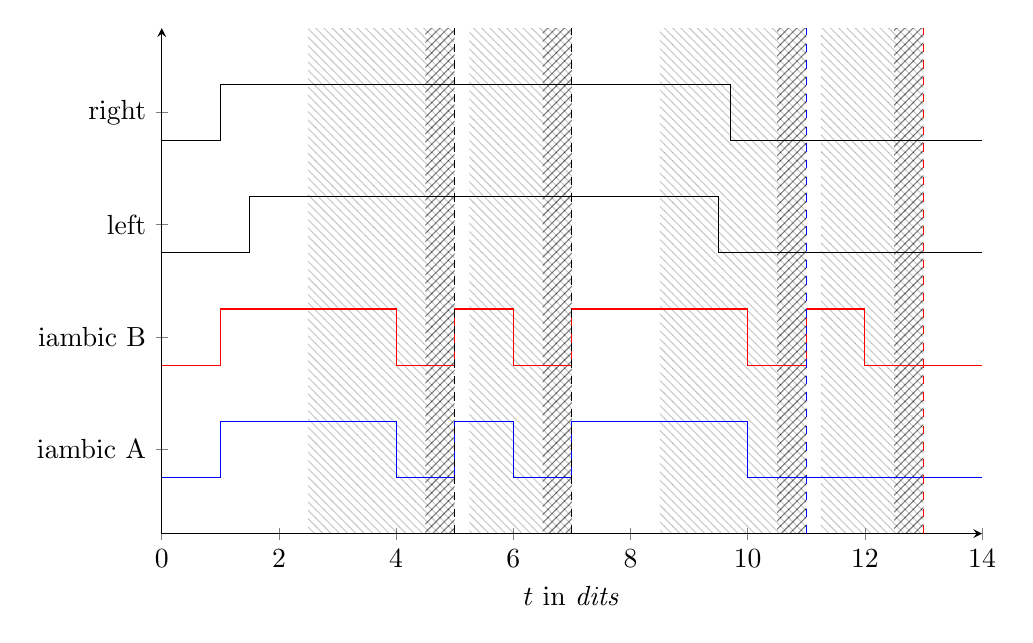
\begin{tikzpicture}
 \begin{axis}[
   axis lines = left,
   xlabel={$t$ in \emph{dits}},
   ytick={1.5,3.5,5.5,7.5},
   yticklabels={{iambic A}, {iambic B}, {left}, {right}}
  ]
  \fill[pattern=north west lines, opacity=0.2] (2.5,0) rectangle (5,9);
  \fill[pattern=north east lines, opacity=0.5] (4.5,0) rectangle (5,9);
  \fill[pattern=north west lines, opacity=0.2] (5.25,0) rectangle (7,9);
  \fill[pattern=north east lines, opacity=0.5] (6.5,0) rectangle (7,9);
  \fill[pattern=north west lines, opacity=0.2] (8.5,0) rectangle (11,9);
  \fill[pattern=north east lines, opacity=0.5] (10.5,0) rectangle (11,9);
  \fill[pattern=north west lines, opacity=0.2] (11.25,0) rectangle (13,9);
  \fill[pattern=north east lines, opacity=0.5] (12.5,0) rectangle (13,9);
  \addplot [mark=none, blue] coordinates {(0,1) (1,1) (1,2) (4,2) (4,1) (5,1) (5,2) (6,2) (6,1) (7,1) (7,2) (10,2) (10,1) (14,1)};
  \addplot [mark=none, red] coordinates {(0,3) (1,3) (1,4) (4,4) (4,3) (5,3) (5,4) (6,4) (6,3) (7,3) (7,4) (10,4) (10,3) (11,3) (11,4) (12,4) (12,3) (14,3)};
  \addplot [mark=none, black] coordinates {(0,5) (1.5,5) (1.5,6) (9.5,6) (9.5,5) (14,5)};
  \addplot [mark=none, black] coordinates {(0,7) (1,7) (1,8) (9.7,8) (9.7,7) (14,7)};
  \addplot +[mark=none, dashed, black] coordinates {(5,0) (5,9)};
  \addplot +[mark=none, dashed, black] coordinates {(7,0) (7,9)};
  \addplot +[mark=none, dashed, blue] coordinates {(11,0) (11,9)};
  \addplot +[mark=none, dashed, red] coordinates {(13,0) (13,9)};
 \end{axis}
\end{tikzpicture}
\end{document}